\chapter{Quantum Logic, Measurement, and Vector Spaces}

Quantum mechanics is not classical mechanics with a little random noise
added. Its unpredictability coexists with exact conservation and reversible
evolution, yet the questions we may ask of a system cannot be separated from
the physical means by which we ask them. The purpose of this first lecture is
to make that difference visible before introducing the formal machinery. We
shall move from the two-slit experiment and reversibility to Heisenberg's
microscope, and only then ask what kind of mathematical object a quantum state
must be.

\section{The Contract of the Course}

People who encounter these lectures on the Internet see the lecturer but not
the audience, and the class can therefore look puzzling. It is neither a
standard undergraduate course nor a graduate course. It belongs to Stanford's
continuing-education program: people from the surrounding community, along
with some people connected to the university, return to theoretical physics
because they want the subject itself.

The age distribution makes the purpose unusually clear. Only a handful of
the roughly one hundred people in the room are under forty; many are over
seventy, a few over eighty, and earlier classes have even included people over
ninety. The audience wants to reach the basic ideas quickly. That does not
mean replacing physics by metaphors. We shall use equations, sometimes hard
equations, but only as much machinery as is needed to get the ideas right.
The aim is a theoretical minimum in the literal sense: efficient,
straightforward, and exact enough to support the next step.

This lecture also belongs to a larger sequence of approximately six
ten-lecture courses. Classical mechanics came first because it supplies the
language of motion, energy, momentum, and time evolution. A course on quantum
entanglement provided an earlier entrance to quantum ideas. The present
course is nevertheless designed to be substantially self-contained. We begin
with the deepest difference between the two subjects: classical and quantum
physics do not organize possibilities according to the same logic.

\section{Classical Randomness Is the Wrong Model}

Quantum mechanics contains unpredictability, but of a very special kind.
Einstein objected that the laws of nature should not amount to a throw of
dice; Bohr's reply was that Einstein should not prescribe what nature may do.
The familiar exchange can be misleading if it suggests that quantum theory
simply inserts a random-number generator into Newton's laws. Let us construct
that classical model first and see why it fails.

Imagine that the moon ordinarily obeys Newton's equation
\begin{equation}
 \mathbf F=m\mathbf a
\end{equation}
together with the law of gravity, but that every tenth of a second an
independent throw of the dice gives it a small extra kick. One outcome pushes
the moon slightly forward, another slightly backward, and most outcomes may
do nothing. Its future orbit would become unpredictable even if its initial
position and velocity were known exactly.

This randomness would leave a characteristic scar. Each kick would change
the energy by a small positive or negative amount. The average change might
vanish, but the accumulated energy would execute a random walk. Exact energy
conservation would be lost.

Quantum evolution does not work that way. Prepare a closed system with a
sharp energy and let it evolve under a time-independent Hamiltonian. A later
energy measurement returns the same energy exactly, even though other
measurement outcomes may be unpredictable.\editorialnote{The qualification
about a closed system and a time-independent Hamiltonian states the standard
condition implicit in the lecture's conservation argument.} Quantum
uncertainty affects some questions while leaving the relevant conservation
law exact. It cannot be represented by occasional violations of an otherwise
classical equation.

\section{Two Slits and the Failure of Classical Alternatives}

The two-slit experiment gives the cleanest first view of the new logic.
Photons, electrons, or neutrons may be used; even a bowling ball has a
quantum wavelength in principle, but the corresponding effect is far too
small to observe. Imagine a source so weak that particles leave one at a
time, perhaps one every five minutes. Each particle passes a barrier and
eventually produces one localized flash or one darkened spot on a screen.

Open only the upper slit. Repeated particles build a broad arrival profile,
which we denote by \(P_1(y)\). Close that slit and open only the lower one.
The second experiment produces another broad profile \(P_2(y)\), displaced
on the screen. If the particles merely received independent classical kicks
while passing the barrier, opening both slits would produce the pointwise sum
\begin{equation}
 P_{\mathrm{cl}}(y)=P_1(y)+P_2(y).
 \label{eq:l01-classical-slit-sum}
\end{equation}
Every particle would use one route or the other, and two available routes
could not make an already accessible point inaccessible.

The experiment gives an interference pattern instead. There are points
\(y_0\) for which
\begin{equation}
 P_{12}(y_0)=0,
 \qquad
 P_1(y_0)>0,
 \qquad
 P_2(y_0)>0.
 \label{eq:l01-destructive-interference}
\end{equation}
Either slit by itself supplies arrivals at \(y_0\); opening both removes them.
The particles may be separated by minutes or years, so the pattern cannot be
attributed to collisions among successive particles.

\begin{figure}[tbp]
\centering

\includegraphics[width=0.76\textwidth]{lecture_01_figure_01.png}
\caption{The completed two-slit interference profile on the board. The
horizontal lobes represent arrival probability along the screen, including
the nodes at which no particles arrive.}
\lectureframe{00:23:55}
\end{figure}

\begin{figure}[tbp]
\centering
\begin{tikzpicture}[>=Latex,scale=0.92]
  \draw[->] (-0.6,0) -- (0.7,0);
  \fill (-0.75,0) circle (2.2pt);
  \node[below] at (-0.75,-0.05) {source};
  \draw[very thick] (1,-2.1) -- (1,-0.35);
  \draw[very thick] (1,0.35) -- (1,2.1);
  \draw[very thick] (1,-0.12) -- (1,0.12);
  \node[above] at (1,2.15) {barrier};
  \draw[->] (1.08,0.25) -- (4.6,1.6);
  \draw[->] (1.08,-0.25) -- (4.6,-1.6);
  \draw[thick] (4.8,-2.2) -- (4.8,2.2);
  \node[above] at (4.8,2.2) {screen};
  \draw[thick,smooth] plot coordinates {
    (4.8,-2.0) (5.0,-1.75) (5.45,-1.55) (5.0,-1.30)
    (4.8,-1.05) (5.05,-0.82) (5.8,-0.55) (5.1,-0.27)
    (4.8,0) (5.1,0.27) (5.8,0.55) (5.05,0.82)
    (4.8,1.05) (5.0,1.30) (5.45,1.55) (5.0,1.75)
    (4.8,2.0)};
  \node[rotate=90] at (6.0,0) {arrival profile};
\end{tikzpicture}
\caption{A clean reconstruction of the board geometry. The measured
probability is built one detection at a time, yet it contains alternating
maxima and nodes.}
\end{figure}

One can invent an elaborate memory hidden in the barrier or screen, but
interference is far too general to be explained by a special mechanism built
for this apparatus. The broad conclusion is unavoidable: the classical rule
for mutually exclusive alternatives is not the fundamental rule. Later we
shall express the replacement in terms of probability amplitudes, which may
cancel before probabilities are formed. At this stage the observed
nonadditivity in Eq.~\eqref{eq:l01-destructive-interference} is enough.

\section{Reversibility and Conservation of Information}

A second route to the same conclusion begins with deterministic motion in a
finite state space. For a two-state coin, one reversible law may leave heads
and tails unchanged,
\begin{equation}
 H\mapsto H,\qquad T\mapsto T,
\end{equation}
while another may interchange them,
\begin{equation}
 H\mapsto T,\qquad T\mapsto H.
\end{equation}
For a fanciful three-sided coin with heads, tails, and feet, consider
\begin{equation}
 H\mapsto T,\qquad T\mapsto F,\qquad F\mapsto H.
 \label{eq:l01-three-cycle}
\end{equation}
Starting from any state, the system cycles forever.

\begin{figure}[tbp]
\centering

\includegraphics[width=0.56\textwidth]{lecture_01_figure_02.png}
\caption{The three-state deterministic cycle. Reversing every arrow gives a
unique route back from each state.}
\lectureframe{00:28:45}
\end{figure}

Let the system run for a million time steps, reverse every arrow, and run for
another million. It returns to its starting point. This is an operational
meaning of reversibility and of information conservation: the present state
still contains everything required to reconstruct the past. We need not even
know the law in detail; we need only a switch that replaces the evolution by
its inverse.

Now add a classical accident. With probability one in a million, suppose the
coin stays put when the rule says to move. A short reversal test may succeed,
but after ten million steps one or more accidents are likely. The reverse
dynamics does not know when the random pauses occurred. In the three-state
example the final reverse run is then no more likely to find the original
state than either of the other two. Classical randomness has destroyed
information.

\section{An Electron Forward and Backward}

Apply the reversal test to a quantum particle. One slit is enough. Send one
electron through it, remove the screen, and do not determine where the
electron goes. After a time \(t\), reverse the dynamics and let the entire
undisturbed system evolve for another time \(t\). In the ideal experiment the
electron returns along the reversed evolution and arrives back at the gun.
Quantum spreading has not acted like a sequence of independent classical
kicks.

Insert an intermediate detector and the result changes. If the detector
records where the electron emerged, then reversing the electron's dynamics
alone does not erase that record. The exact return test fails. In modern
language, the electron has become correlated with degrees of freedom in the
detector; the closed combined system may still evolve reversibly, but the
electron can no longer be treated as though nothing else carries its
history.\editorialnote{This closed-system formulation sharpens the lecture's
contrast without adding a new formalism.}

The classical contrast is deliberately mundane. Looking at a coin---the
lecture uses a Chilean peso---need not turn heads into tails. If sufficiently
energetic light is used, it can of course knock the coin over, but classical
physics allows the illumination to be made arbitrarily gentle while still
revealing the state. An intermediate classical observation therefore need
not spoil the reversal experiment. Quantum measurement admits no analogous
limit in which a perfectly sharp observation has an arbitrarily small effect.

The two-slit experiment tells the same story. Interference survives only if
nothing records which slit the electron used. The recorder need not be a
human observer. A gas molecule, another electron, or any other physical
degree of freedom may retain the path information. If the upper path changes
one molecule and the lower path changes another, then the alternatives leave
distinguishable records. The interference disappears and the observed
probabilities reduce to the classical sum in
Eq.~\eqref{eq:l01-classical-slit-sum}.

\begin{classroomqa}
\audiencequestion{If a particle passes through one slit and is deflected,
does momentum conservation not give the plate an opposite recoil, thereby
recording the path?\lecturetimestamp{00:44:30--00:44:47}}
\lecturerresponse{The recoil is real, but a physical kick is not
automatically a readable record. A plate localized well enough to define the
slits has an intrinsically broad momentum distribution. The recoil shifts
that distribution. If the shift is small compared with its width, the
post-collision momentum does not reveal whether the kick occurred.}
\end{classroomqa}

\begin{figure}[tbp]
\centering

\includegraphics[width=0.76\textwidth]{lecture_01_figure_03.png}
\caption{The plate's broad momentum profile and its small recoil-induced
shift. The two nearly coincident curves are the part of the board relevant to
the argument.}
\lectureframe{00:46:30}
\end{figure}

\begin{figure}[tbp]
\centering
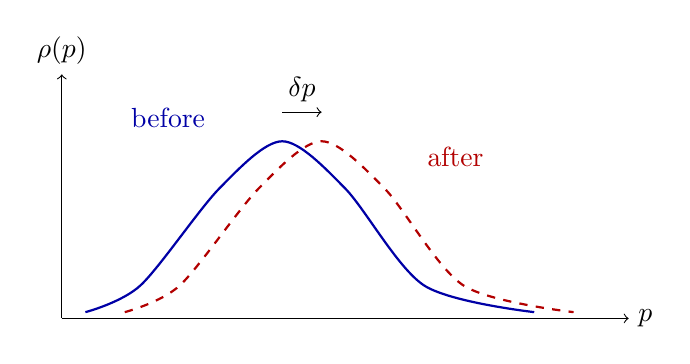
\begin{tikzpicture}[scale=1.0]
  \draw[->] (0,0) -- (7.2,0) node[right] {$p$};
  \draw[->] (0,0) -- (0,3.1) node[above] {$\rho(p)$};
  \draw[thick,blue!65!black] plot[smooth] coordinates {
    (0.3,0.08) (1.0,0.42) (2.0,1.65) (2.8,2.25)
    (3.6,1.65) (4.6,0.42) (6.0,0.08)};
  \draw[thick,dashed,red!70!black] plot[smooth] coordinates {
    (0.8,0.08) (1.5,0.42) (2.5,1.65) (3.3,2.25)
    (4.1,1.65) (5.1,0.42) (6.5,0.08)};
  \draw[->] (2.8,2.62) -- (3.3,2.62);
  \node[above] at (3.05,2.62) {$\delta p$};
  \node[blue!65!black] at (1.35,2.55) {before};
  \node[red!70!black] at (5.0,2.05) {after};
\end{tikzpicture}
\caption{The recoil becomes a path record only when the shift
\(\delta p\) is distinguishable relative to the initial width.}
\end{figure}

The uncertainty principle closes the apparent loophole. Making the plate's
momentum sharp enough to resolve a tiny kick makes its position correspondingly
uncertain, so the slit geometry itself becomes blurred. The apparatus cannot
simultaneously define the paths sharply and record an arbitrarily small
path-dependent recoil.

\section{Why Classical Uncertainty Is Not Fundamental}

Before deriving the microscope argument, distinguish quantum uncertainty
from an ordinary statistical cloud. A Brownian particle is knocked by
surrounding molecules, and an ensemble of such particles spreads in position
and velocity. In classical physics this uncertainty reflects incomplete
observation. With a better microscope, a more accurate detector, and gentler
illumination, one imagines determining the position and velocity of each
particle as accurately as desired.

Quantum mechanics contains a logical obstruction to that refinement. It is
not merely that our apparatus is coarse or expensive. A procedure that makes
position sharper necessarily changes what can be said about momentum.
Heisenberg first encountered this through abstract mathematics, where the
operations corresponding to position and momentum do not commute. The
microscope thought experiment supplies the physical illustration.

\section{Heisenberg's Microscope}

To locate a particle optically, scatter light from it and focus the scattered
wave into an image. The required chain begins with the energy of one photon,
\begin{equation}
 E=hf=\hbar\omega,
 \qquad
 \omega=2\pi f,
 \qquad
 \hbar=\frac{h}{2\pi}.
 \label{eq:l01-photon-energy}
\end{equation}
Visible light has a frequency of order \(10^{15}\,\mathrm{Hz}\). Light also
carries momentum: an absorbed beam heats a door because it carries energy
and can push the door because it carries momentum.

For a nonrelativistic particle,
\begin{equation}
 E_{\mathrm{kin}}=\frac{p^2}{2m}=\frac12 pv,
\end{equation}
whereas for light relativity gives
\begin{equation}
 E=cp,\qquad p=\frac{E}{c}.
 \label{eq:l01-light-momentum}
\end{equation}
One cycle has period \(T=1/f\), and in that time a light wave advances by one
wavelength. Hence
\begin{equation}
 c=\frac{\lambda}{T}=\lambda f,
 \qquad
 f=\frac{c}{\lambda}.
\end{equation}
Combining this with Eqs.~\eqref{eq:l01-photon-energy} and
\eqref{eq:l01-light-momentum} gives
\begin{equation}
 p_\gamma=\frac{hf}{c}=\frac{h}{\lambda}.
 \label{eq:l01-de-broglie}
\end{equation}
Short wavelength means large photon momentum.

\begin{figure}[tbp]
\centering

\includegraphics[width=0.78\textwidth]{lecture_01_figure_04.png}
\caption{The board at the decisive step: \(E=hf=\hbar\omega\),
\(p=h/\lambda\), \(c/\lambda=f\), and the imaging condition
\(\lambda<\Delta x\).}
\lectureframe{01:03:18}
\end{figure}

An image cannot resolve detail much smaller than its wavelength. To locate a
particle on a scale \(\Delta x\), the probe must therefore satisfy, at the
order-of-magnitude level,
\begin{equation}
 \lambda\lesssim\Delta x.
 \label{eq:l01-resolution}
\end{equation}
But the photon used to obtain that resolution carries momentum
\(h/\lambda\). When it scatters from the particle, the unknown scattering
direction gives the particle an uncertain kick of the same order:
\begin{equation}
 \Delta p_{\mathrm{kick}}\sim\frac{h}{\lambda}.
 \label{eq:l01-kick}
\end{equation}
Equations~\eqref{eq:l01-resolution} and \eqref{eq:l01-kick} give the
heuristic scale
\begin{equation}
 \Delta x\,\Delta p_{\mathrm{kick}}\gtrsim h
 \qquad\text{(order of magnitude)}.
\end{equation}
This is not the later sharp inequality with its convention-dependent
numerical factor; it is the microscope logic that motivates it.

\begin{figure}[tbp]
\centering

\includegraphics[width=0.72\textwidth]{lecture_01_figure_05.png}
\caption{A short-wavelength photon localizes the particle sharply, then
scatters in an uncontrolled direction and transfers momentum.}
\lectureframe{01:04:45}
\end{figure}

Why does the same argument not seem fatal classically? A classical light wave
may be divided into arbitrarily small amounts of energy while its wavelength
is held fixed. One could imagine forming the same sharp image with an
arbitrarily weak wave. Quantum light comes in indivisible packets. At a fixed
wavelength the smallest available probe is one photon, and that photon
already carries \(h/\lambda\). A precise position measurement cannot be made
arbitrarily gentle. A gentle measurement is possible only by using a long
wavelength and accepting a coarse position.

\section{Measuring Velocity Gently}

After the break, a question asks how velocity can be measured at all. The
answer is to use two deliberately imprecise position measurements and allow a
long time between them. Suppose the particle's mass is known, so that
measuring velocity also determines its nonrelativistic momentum.

Use a long-wavelength photon for the first observation. It gives only
\begin{equation}
 x_1=x+O(\lambda),
\end{equation}
but its momentum is small enough that the particle receives only a gentle
kick. Wait for a time \(t\), then make a second long-wavelength observation:
\begin{equation}
 x_2=x+vt+O(\lambda).
\end{equation}
The inferred displacement and velocity are
\begin{align}
 d&=x_2-x_1=vt+O(\lambda),\\
 v_{\mathrm{meas}}&=\frac{d}{t}
                   =v+O\!\left(\frac{\lambda}{t}\right).
 \label{eq:l01-gentle-velocity}
\end{align}
No matter how large \(\lambda\) is, the measurement contribution
\(\lambda/t\) can be made small by waiting long enough.

\begin{figure}[tbp]
\centering

\includegraphics[width=0.76\textwidth]{lecture_01_figure_06.png}
\caption{The two coarse position readings and the resulting velocity
estimate \(v=d/t\) with uncertainty of order \(\lambda/t\).}
\lectureframe{01:13:15}
\end{figure}

The tradeoff has not disappeared. Velocity is determined accurately only
while position remains uncertain on the large scale \(\lambda\). The method
does not assign both a sharp position and a sharp momentum at one instant.

\begin{classroomqa}
\audiencequestion{Does the term \(\lambda/t\) include every source of
uncertainty in this velocity experiment?\lecturetimestamp{01:14:07--01:16:16}}
\lecturerresponse{No. It describes the uncertainty contributed by the two
coarse position readings. The original preparation supplies another
uncertainty, and the complete accounting requires keeping both. A fixed
reference object such as a wall can have its mean position determined by
averaging many gentle photon measurements over a long time. The detailed
follow-up is deferred rather than answered by pretending that
\(\lambda/t\) is the whole uncertainty principle.}
\end{classroomqa}

\section{Classical States Are Points in Phase Space}

The experiments point to a failure of classical logic, and the failure
appears at the most elementary question: what is a state? For a classical
coin the alternatives \(H\) and \(T\) are points in a set. For a die the set
has six points. For one classical particle, a state is a point in phase
space,
\begin{equation}
 (x,p),
\end{equation}
and for many particles it is the corresponding list of all positions and
momenta. Dynamics is a flow carrying one point of this set into another.

If the apparatus is coarse, we may describe our knowledge by a probability
density on phase space,
\begin{equation}
 \rho(x,p)\geq0,
 \qquad
 \int dx\,dp\,\rho(x,p)=1.
\end{equation}
The distribution may be concentrated in a small region and fall away from
its center. Classical logic treats this as incomplete knowledge, not as the
maximal possible specification of the state. More delicate, less disturbing
measurements can in principle concentrate \(\rho\) more closely around one
phase-space point.

That conclusion is exactly what quantum mechanics refuses. A quantum state
requires more structure than a point-set description supplies. Of course any
collection of states can be regarded as a set in the formal mathematical
sense; the claim is that set membership and classical probability are not
the natural operations that organize quantum alternatives. The state space
must support linear combinations.

\section{Complex Vector Spaces and Ket Vectors}

A vector space is a collection of objects called vectors together with two
operations. Vectors may be added, and they may be multiplied by scalars. For
the spaces used in quantum mechanics, the scalars are complex numbers. Thus
if \(\ket a,\ket b\in V\) and \(\alpha,\beta\in\mathbb C\), then
\begin{equation}
 \alpha\ket a+\beta\ket b\in V.
 \label{eq:l01-linear-combination}
\end{equation}
This closure under linear combinations is the first mathematical departure
from a classical list of alternatives. Multiplying heads by
\(2+4i\) has no meaning in the classical two-point state space; multiplying
a ket vector by a complex scalar is a basic operation.

\begin{figure}[tbp]
\centering

\includegraphics[width=0.74\textwidth]{lecture_01_figure_07.png}
\caption{Ket-vector addition and a general complex linear combination. The
result is another ket vector in the same vector space.}
\lectureframe{01:32:35}
\end{figure}

Dirac denoted these vectors by kets such as \(\ket a\), half of a bracket.
The complementary half will be a bra, and a bra next to a ket makes a
bracket. That structure comes later; for the moment the notation only marks
an abstract vector.

The word \emph{vector} must not be confused with an arrow in ordinary
three-dimensional space. To keep the distinction visible, call the familiar
arrow a \emph{pointer}. A pointer has a length and a spatial direction. It
can be multiplied by a real number and added to another pointer by the
parallelogram rule, so pointers form a vector space over \(\mathbb R\).
Quantum state vectors are more general and form spaces over \(\mathbb C\).

The lecture occasionally uses \emph{Hilbert space} while introducing this
linear structure. Strictly, a complex vector space becomes a Hilbert space
only after an inner product and an appropriate completeness condition are
supplied. Those additions have not yet been introduced; at this stage we
need only the two linear operations.

\section{Functions as Vectors}

Consider complex-valued functions of one real variable,
\begin{equation}
 \psi(x)=\psi_R(x)+i\psi_I(x).
\end{equation}
The argument \(x\) is real; the value of the function may be complex. Given
two such functions and a complex number \(\alpha\), define
\begin{align}
 (\psi+\phi)(x)&=\psi(x)+\phi(x),\\
 (\alpha\psi)(x)&=\alpha\psi(x).
\end{align}
Both operations produce new complex-valued functions, so any chosen class of
functions closed under these operations forms a complex vector space. Real
functions similarly form a vector space over \(\mathbb R\), but not over
\(\mathbb C\), because multiplying a real function by \(i\) takes it out of
the real-valued collection.

\begin{figure}[tbp]
\centering

\includegraphics[width=0.78\textwidth]{lecture_01_figure_08.png}
\caption{A complex function resolved into real and imaginary parts, beneath
the ket-vector linear-combination rule.}
\lectureframe{01:36:45}
\end{figure}

Function spaces are the examples that motivated Hilbert's work and will
become central to wave mechanics. Questions of inner products,
normalization, and which functions are admissible are deliberately left for
later.

\section{Columns and Dimension}

A finite-dimensional example is a column of \(n\) complex numbers. For
\(n=4\),
\begin{equation}
 A=
 \begin{pmatrix}
  a_1\\a_2\\a_3\\a_4
 \end{pmatrix},
 \qquad
 B=
 \begin{pmatrix}
  b_1\\b_2\\b_3\\b_4
 \end{pmatrix}.
\end{equation}
Addition and scalar multiplication are componentwise:
\begin{align}
 A+B&=
 \begin{pmatrix}
  a_1+b_1\\a_2+b_2\\a_3+b_3\\a_4+b_4
 \end{pmatrix},&
 \alpha A&=
 \begin{pmatrix}
  \alpha a_1\\\alpha a_2\\\alpha a_3\\\alpha a_4
 \end{pmatrix}.
 \label{eq:l01-column-operations}
\end{align}
No multiplication of one vector by another has been defined. Only addition
of vectors and multiplication of a vector by a scalar are needed here.

\begin{figure}[tbp]
\centering

\includegraphics[width=0.76\textwidth]{lecture_01_figure_09.png}
\caption{Componentwise addition and complex scalar multiplication for
four-component columns.}
\lectureframe{01:42:00}
\end{figure}

Columns of a fixed length \(n\) form an \(n\)-dimensional complex vector
space. Pairs, quadruples, and infinite columns each give their own spaces;
throwing columns of every possible length into one collection does not give
one vector space under these rules, because no addition has been defined
between a two-component and a three-component column. The entries may be
viewed as components, just as the entries of a spatial pointer are its
components along chosen axes. One may also regard a column as a function of
its discrete index, but that abstraction is postponed.

We have not yet explained in what physical sense a state is represented by
such a vector. The present task is only to learn the operations before
applying them to quantum systems.

\begin{classroomqa}
\audiencequestion{At this stage, is the vector-space discussion supposed to
sound like mumbo jumbo?\lecturetimestamp{01:44:52--01:45:10}}
\lecturerresponse{Its physical use has not yet been supplied, so the
abstraction is expected to feel unmotivated. The definitions themselves are
nevertheless precise: vectors can be added and multiplied by complex
numbers. The next lectures will connect those operations to physical
states.}
\end{classroomqa}

The analogy with logic is worth retaining. Classical Boolean operations act
on sets: \emph{and} corresponds to intersection, while \emph{or} corresponds
to union. The lecture momentarily interchanges the two and corrects the
order. Quantum logic will be organized by subspaces and linear operations
rather than by ordinary unions of alternatives. That is why vector spaces
are not optional mathematical decoration.

\section{Complex Conjugation}

The complex numbers themselves form a one-dimensional vector space over
\(\mathbb C\). They also carry an operation that will be indispensable when
inner products are introduced. Write
\begin{equation}
 z=x+iy.
\end{equation}
Its complex conjugate is
\begin{equation}
 z^\ast=x-iy.
\end{equation}
Geometrically, conjugation reflects the point in the complex plane across
the real axis. Algebraically,
\begin{align}
 z^\ast z
 &=(x-iy)(x+iy)\\
 &=x^2+y^2
 =|z|^2.
 \label{eq:l01-complex-magnitude}
\end{align}
The cross terms cancel and \(i(-i)=1\), leaving the squared distance from the
origin.

\begin{figure}[tbp]
\centering

\includegraphics[width=0.74\textwidth]{lecture_01_figure_10.png}
\caption{The board calculation \(zz^\ast=(x+iy)(x-iy)=x^2+y^2\).}
\lectureframe{01:49:30}
\end{figure}

\begin{figure}[tbp]
\centering
\begin{tikzpicture}[>=Latex,scale=0.95]
  \draw[->] (-0.3,0) -- (5.2,0) node[right] {$\operatorname{Re}z$};
  \draw[->] (0,-2.4) -- (0,2.7) node[above] {$\operatorname{Im}z$};
  \draw[dashed] (3.5,-1.7) -- (3.5,1.7);
  \draw[dashed] (0,1.7) -- (3.5,1.7);
  \draw[dashed] (0,-1.7) -- (3.5,-1.7);
  \draw[thick,->,blue!65!black] (0,0) -- (3.5,1.7)
    node[above right] {$z=x+iy$};
  \draw[thick,->,red!70!black] (0,0) -- (3.5,-1.7)
    node[below right] {$z^\ast=x-iy$};
  \node[below] at (3.5,0) {$x$};
  \node[left] at (0,1.7) {$y$};
  \node[left] at (0,-1.7) {$-y$};
\end{tikzpicture}
\caption{Complex conjugation is reflection across the real axis; both
vectors have magnitude \(\sqrt{x^2+y^2}\).}
\end{figure}

Conjugation is best regarded as a map from complex numbers back to complex
numbers, not merely as a trick for simplifying products. The next lecture
will extend the vector-space language, introduce operators, Hermitian
operators, and eigenvalues, and begin applying this machinery to quantum
systems.
